\documentclass{article}
\usepackage{amsmath}
\usepackage{graphicx}
\usepackage{epstopdf}
\usepackage{float}
\usepackage{subcaption}
\usepackage{tikz}
\usepackage{ifthen}
\usepackage{color}
\usepackage{graphicx}
\usepackage{hyperref}
\newcommand{\myScale}{0.56}
\title{CSL603 - Lab 3\\Multi Layer Perceptron}
\author{Aditya Gupta\\2015CSB1003\\Soumyadeep Roy\\2015CSB1035}
\begin{document}
\maketitle
\section{2-Dimensional 3-Class Classification problem}
\subsection{Goal} Study the changes to the 
\begin{itemize}
\item decision boundary and 
\item the training error
\end{itemize} with respect to parameters such as 
\begin{itemize}
\item number of training iterations,
\item number of hidden layer neurons and
\item finally the learning rate
\end{itemize}
\subsection{MLP Training}
During forward pass, we made $z_h=\sigma(w_h^Tx)$, $y'_k=\exp(v_k^Tz)/\sum_{k'=1}^K \exp(v_{k'}^Tz)$ (The weights and points had different orientation to what discussed in class, therefore an appropriate formula equivalent to these was used.)
During backpropagation, for a particular point we used $$\Delta v_{hk}=\underbrace{\eta(y'_k-y_k)}_{\text{Common for a particular } k}z_h$$, $$\Delta w_{jh}=\underbrace{\eta\left(\sum_k(y'_k-y_k)v_{hk}\right)z_h(1-z_h)}_{\text{Common for a particular }h}x_j$$ (Various values were calculated only once which were common for a particular $k$ for $\Delta v_{hk}$ and these were further used in case of $\Delta w_{jh}$, moreover the common values in case of $\Delta w_{jh}$ for a particular $h$ were also calculated only once.)
\subsection{Training Error}
The training error was calculated as $E(w,v)=-\sum_{k=1}^K y_k\log y'_k$ for a particular point that was trained in this epoch.
\subsection{MLP Testing}
The similar formulas as for MLP training were used but here, instead we had multiple points, so an appropriate form was used (The bias term was introduced differently which in this case would be a column vector, rest was same).
\subsection{Observations}
\subsubsection{Varying the number of hidden layer nodes}
The following figures depict the change in the sum of squared error vs. the number of training iterations for a particular $\eta$ value and varying the number of hidden layer nodes in powers of $2$:
\begin{figure}[H]
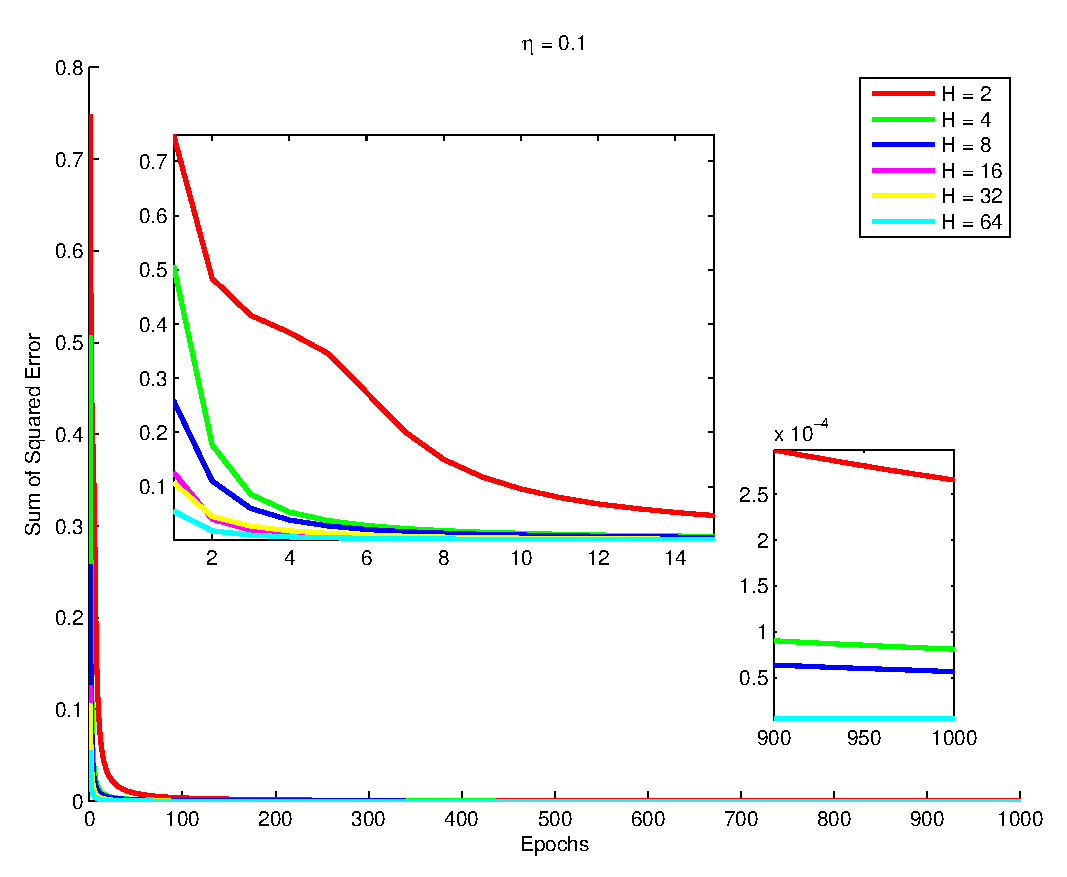
\includegraphics[scale=\myScale]{{../eps2/eta0.100000}.eps}
\caption{Change in Sum of Squared Error vs the Training Iterations for different values of H. $\eta=0.1$}
\label{fig:fig1}
\end{figure}
\begin{figure}[H]
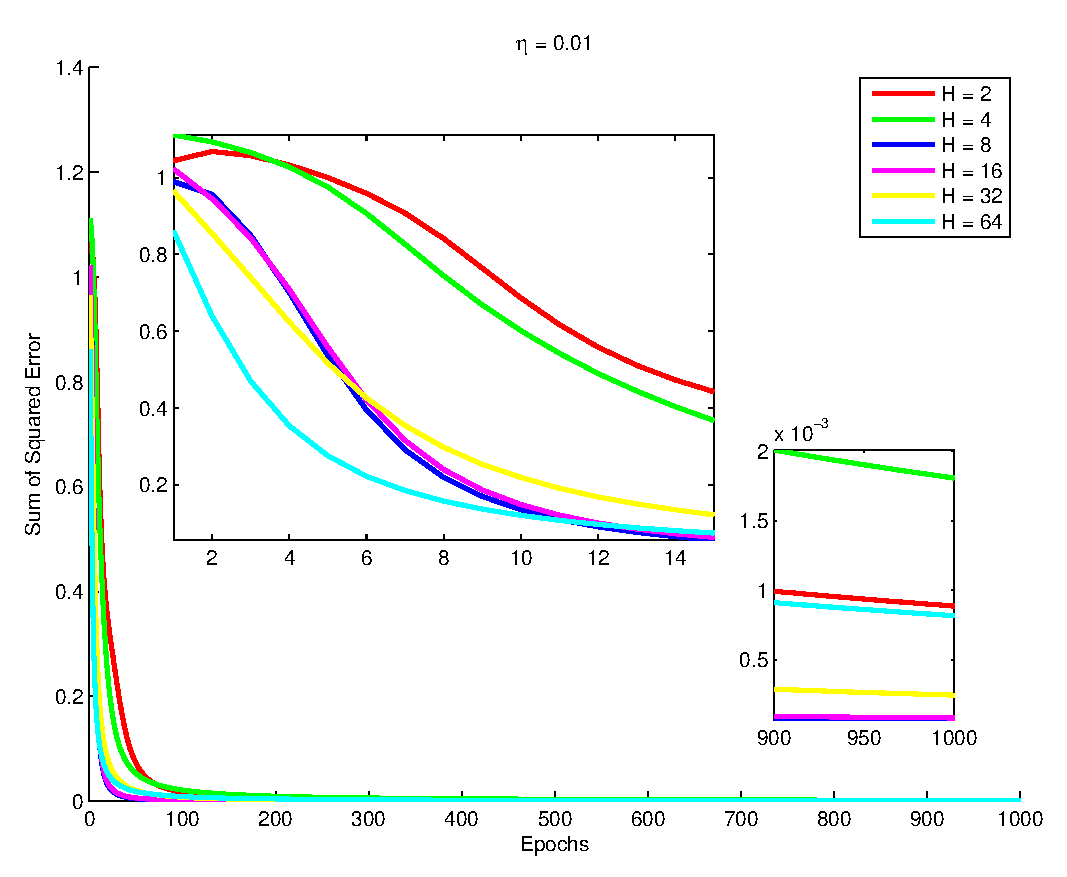
\includegraphics[scale=\myScale]{{../eps2/eta0.010000}.eps}
\caption{Change in Sum of Squared Error vs the Training Iterations for different values of H. $\eta=0.01$}
\label{fig:fig2}
\end{figure}
\begin{figure}[H]
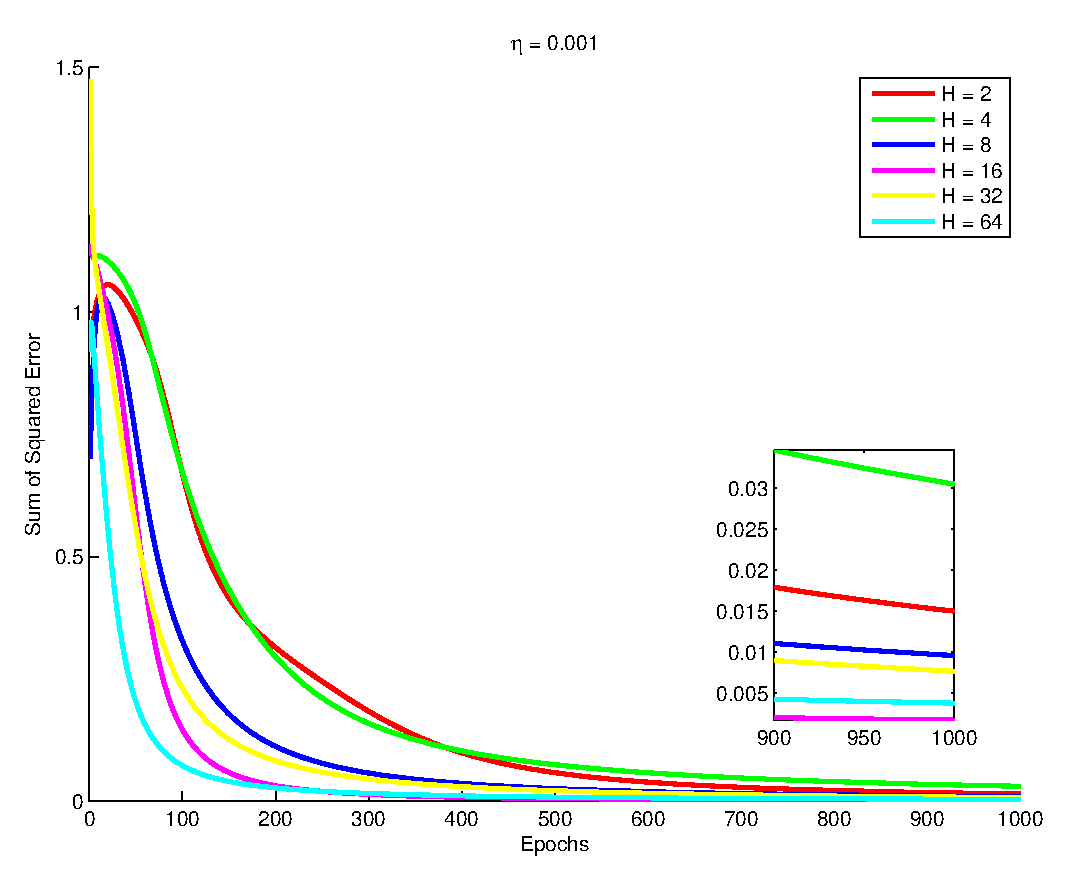
\includegraphics[scale=\myScale]{{../eps2/eta0.001000}.eps}
\caption{Change in Sum of Squared Error vs the Training Iterations for different values of H. $\eta=0.001$}
\label{fig:fig3}
\end{figure}
\begin{figure}[H]
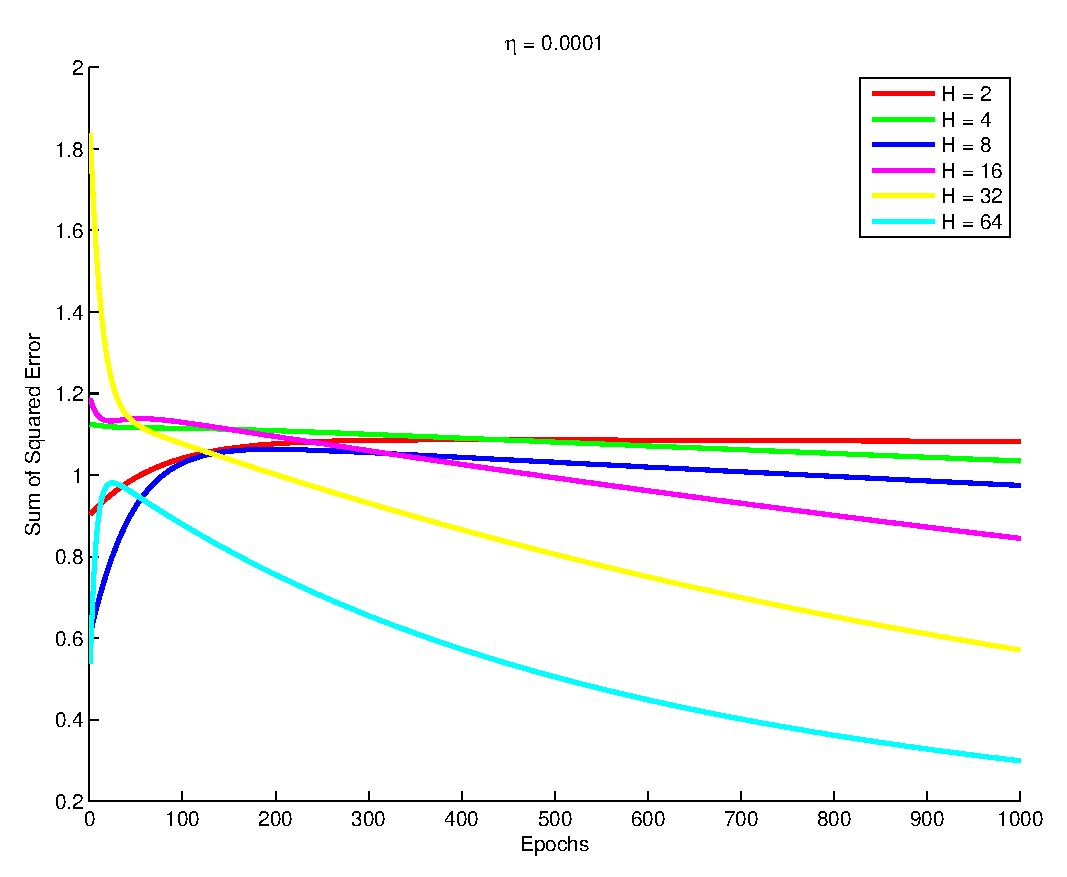
\includegraphics[scale=\myScale]{{../eps2/eta0.000100}.eps}
\caption{Change in Sum of Squared Error vs the Training Iterations for different values of H. $\eta=0.0001$}
\label{fig:fig4}
\end{figure}
\begin{figure}[H]
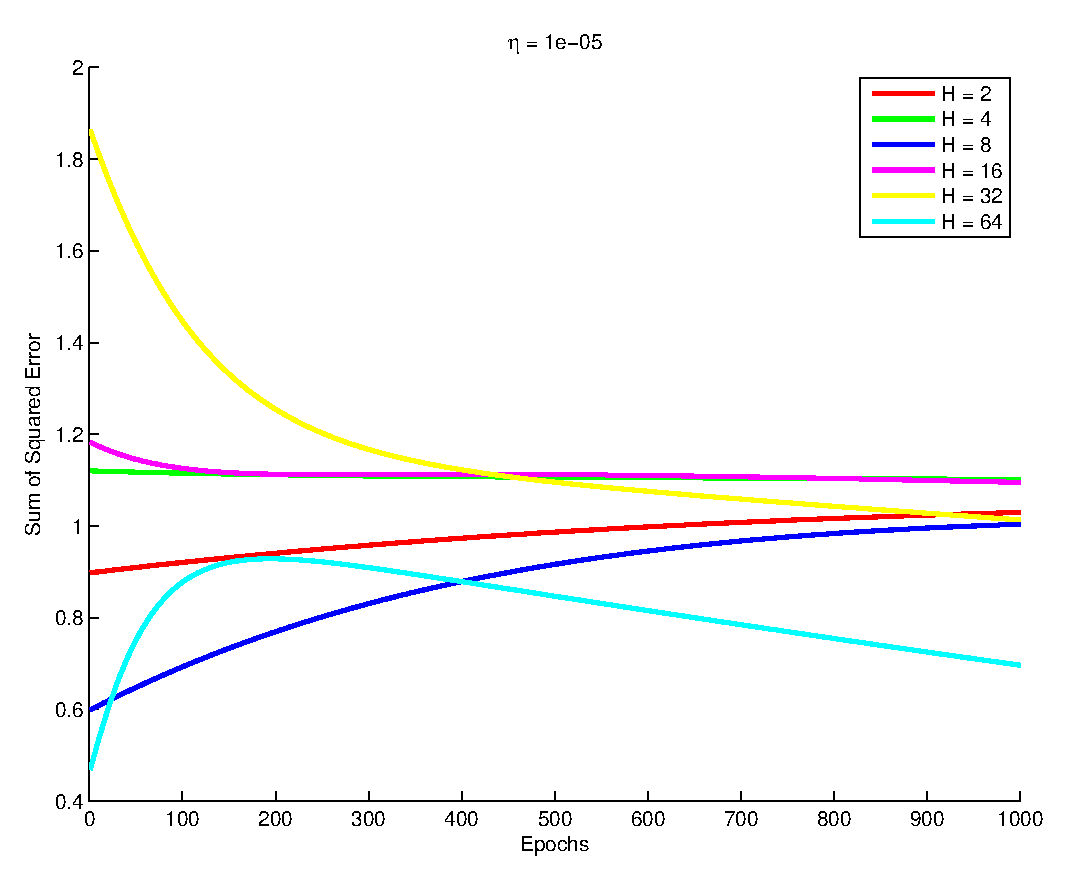
\includegraphics[scale=\myScale]{{../eps2/eta0.000010}.eps}
\caption{Change in Sum of Squared Error vs the Training Iterations for different values of H. $\eta=0.00001$}
\label{fig:fig5}
\end{figure}

\subsubsection{Varying the learning rate}
The following figures depict the change in the sum of squared error vs. the number of training iterations for a particular value of $H$ and varying the $\eta$:
\begin{figure}[H]
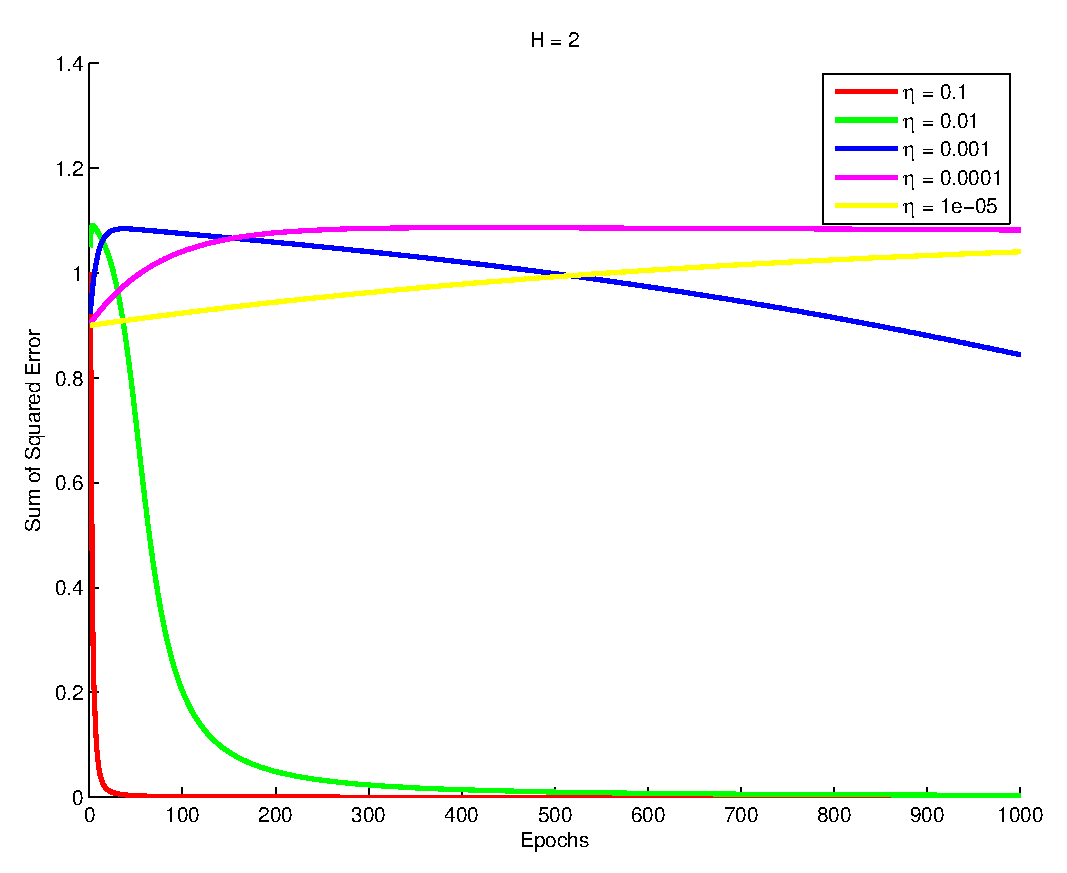
\includegraphics[scale=\myScale]{../eps2/H2.eps}
\caption{Change in Sum of Squared Error vs the Training Iterations for different values 
of $\eta$. $H=2$}
\label{fig:fig6}
\end{figure}
\begin{figure}[H]
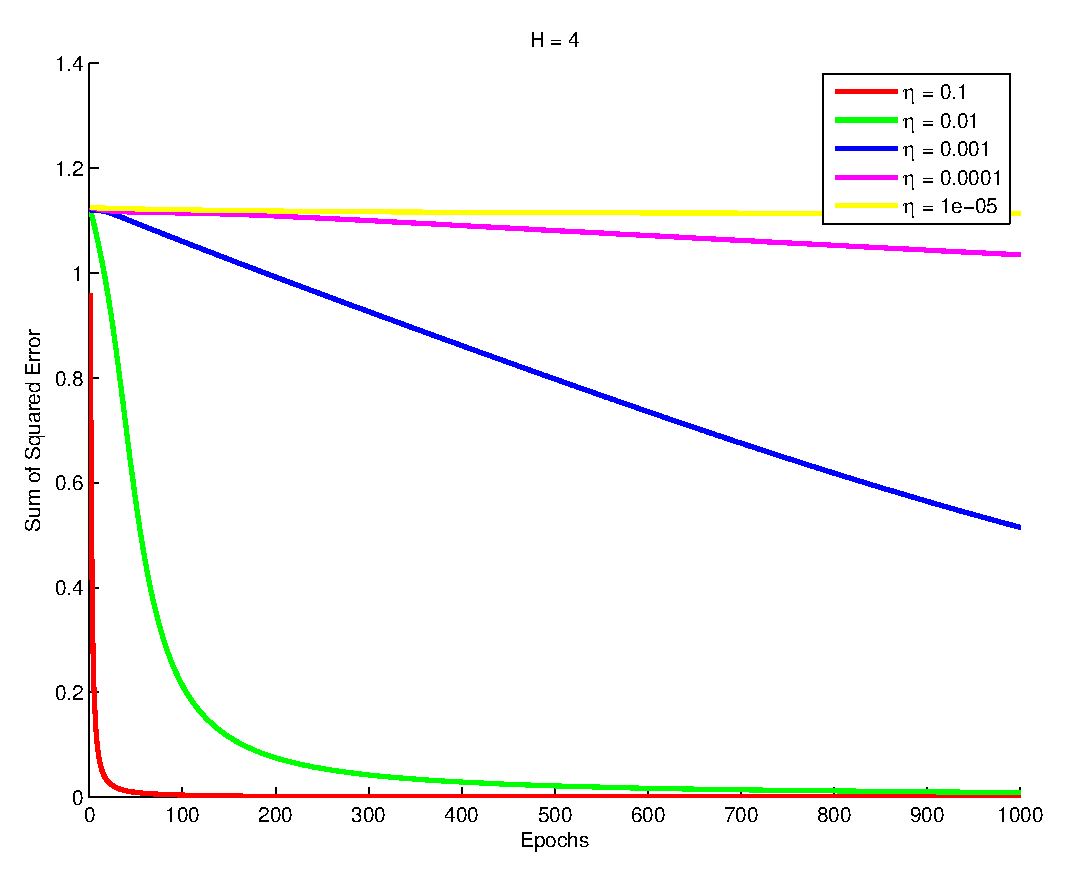
\includegraphics[scale=\myScale]{../eps2/H4.eps}
\caption{Change in Sum of Squared Error vs the Training Iterations for different values of $\eta$. $H=4$}
\label{fig:fig7}
\end{figure}
\begin{figure}[H]
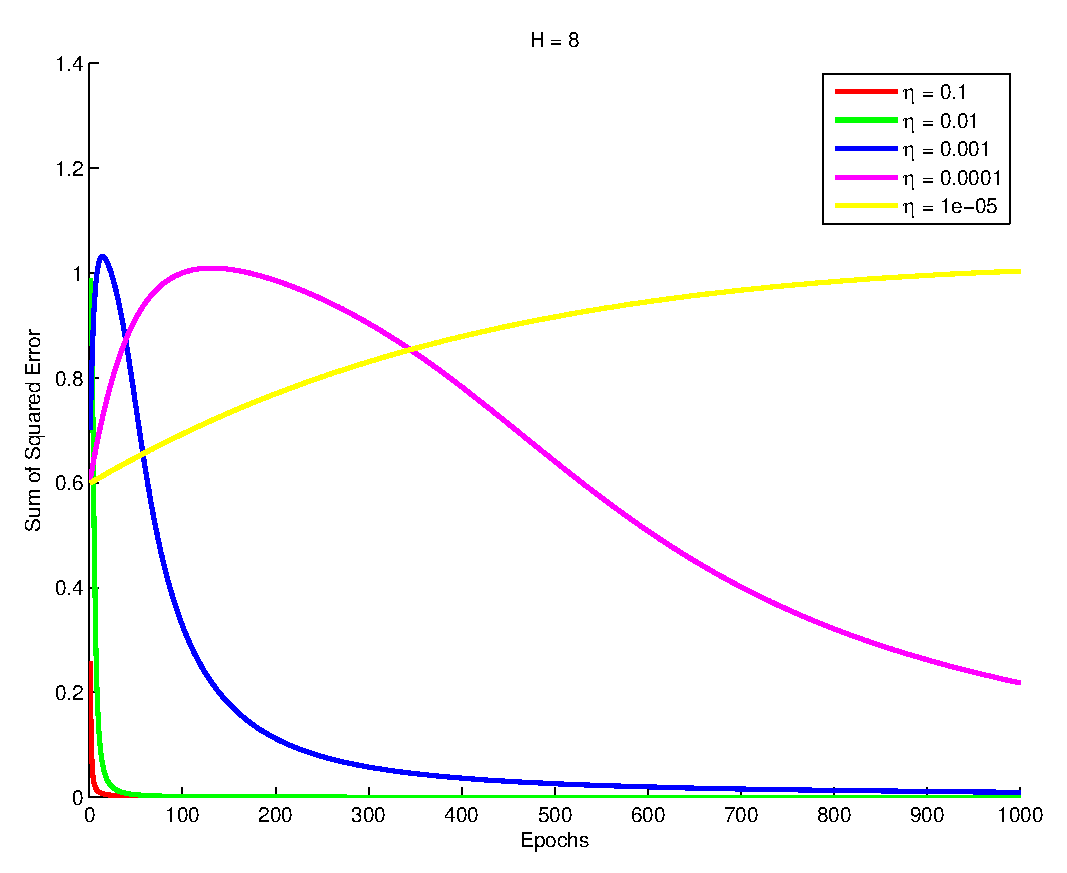
\includegraphics[scale=\myScale]{../eps2/H8.eps}
\caption{Change in Sum of Squared Error vs the Training Iterations for different values of $\eta$. $H=8$}
\label{fig:fig8}
\end{figure}
\begin{figure}[H]
\includegraphics[scale=\myScale]{../eps2/H16.eps}
\caption{Change in Sum of Squared Error vs the Training Iterations for different values of $\eta$. $H=16$}
\label{fig:fig9}
\end{figure}
\begin{figure}[H]
\includegraphics[scale=\myScale]{../eps2/H32.eps}
\caption{Change in Sum of Squared Error vs the Training Iterations for different values of $\eta$. $H=32$}
\label{fig:fig10}
\end{figure}
\begin{figure}[H]
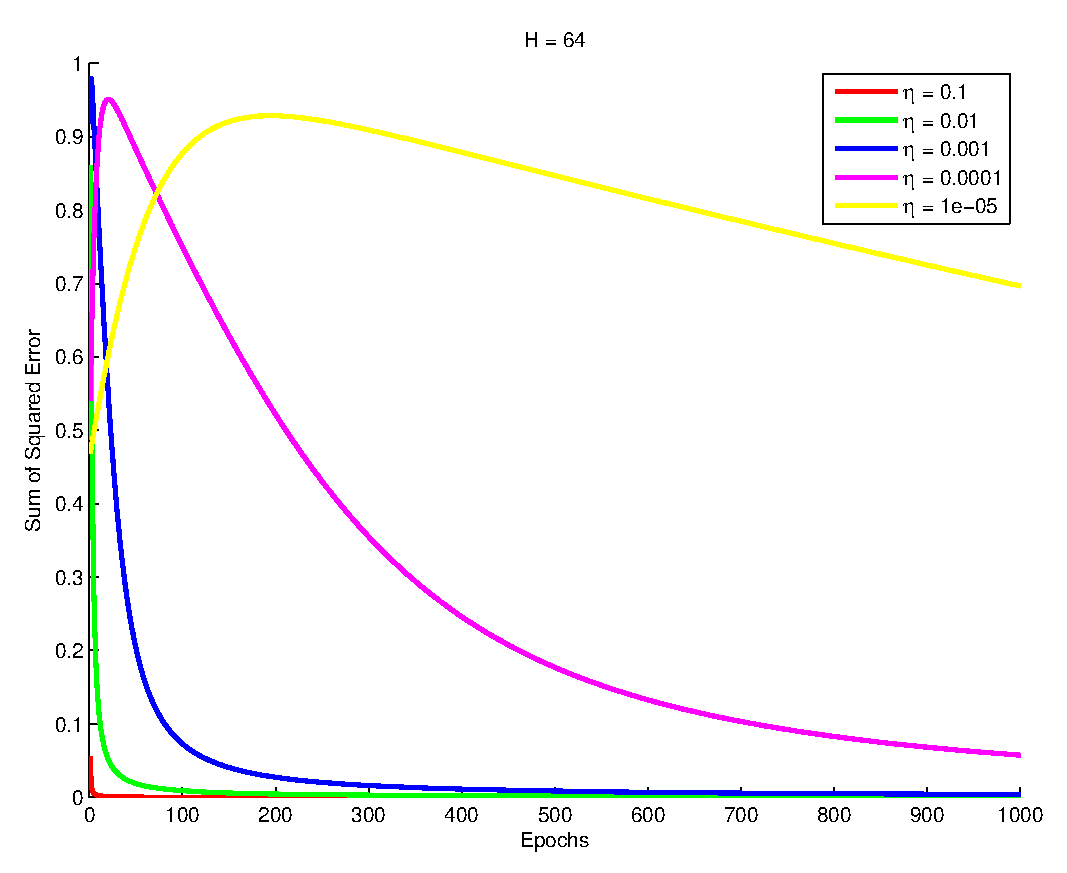
\includegraphics[scale=\myScale]{../eps2/H64.eps}
\caption{Change in Sum of Squared Error vs the Training Iterations for different values of $\eta$. $H=64$}
\label{fig:fig11}
\end{figure}

\subsubsection{Varying the training iterations}
The observations for the change in the sum of squared error by varying the training iterations can be made through the previous graphs.

\subsubsection{Change in Decision Boundary}
The change in decision boundaries for various values of $H$  and $\eta$ can be seen in the following graphs. Here red dots represent Class 1, green pluses represent Class 2 and blue circles represent Class 3.

\begin{figure}[H]
\minipage{0.32\textwidth}
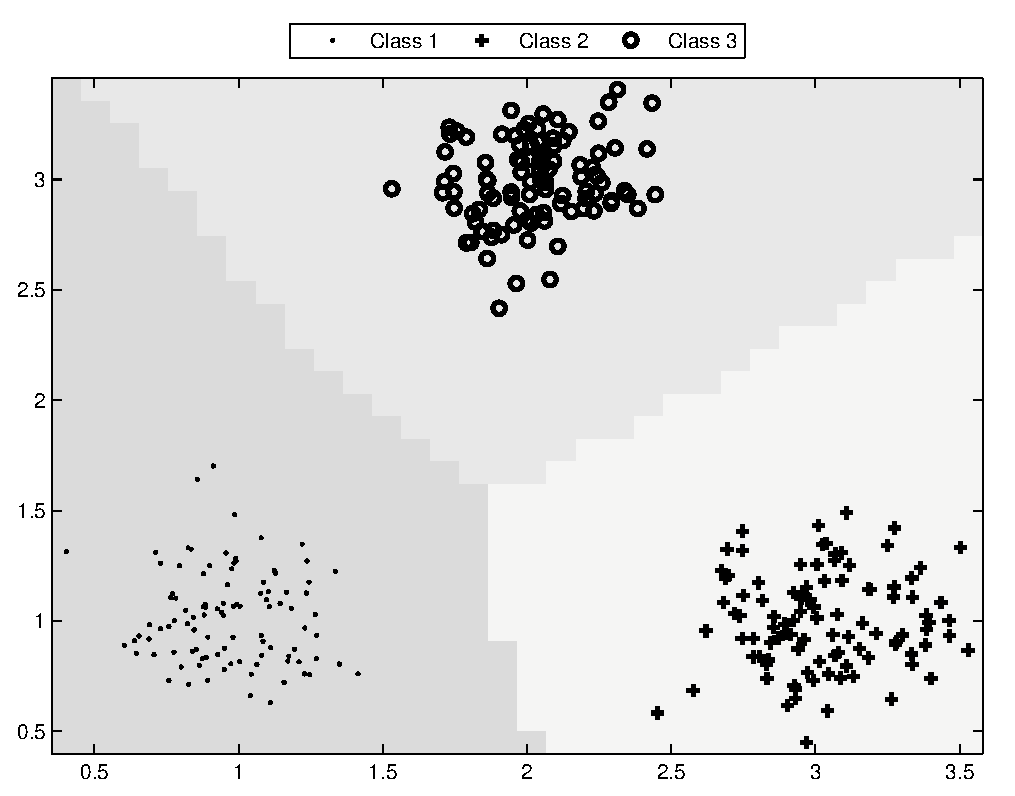
\includegraphics[scale=0.25]{{../eps/fig2_H2_eta0.010000}.eps}
\subcaption{ $H=2$}
\endminipage\hfill
\minipage{0.32\textwidth}
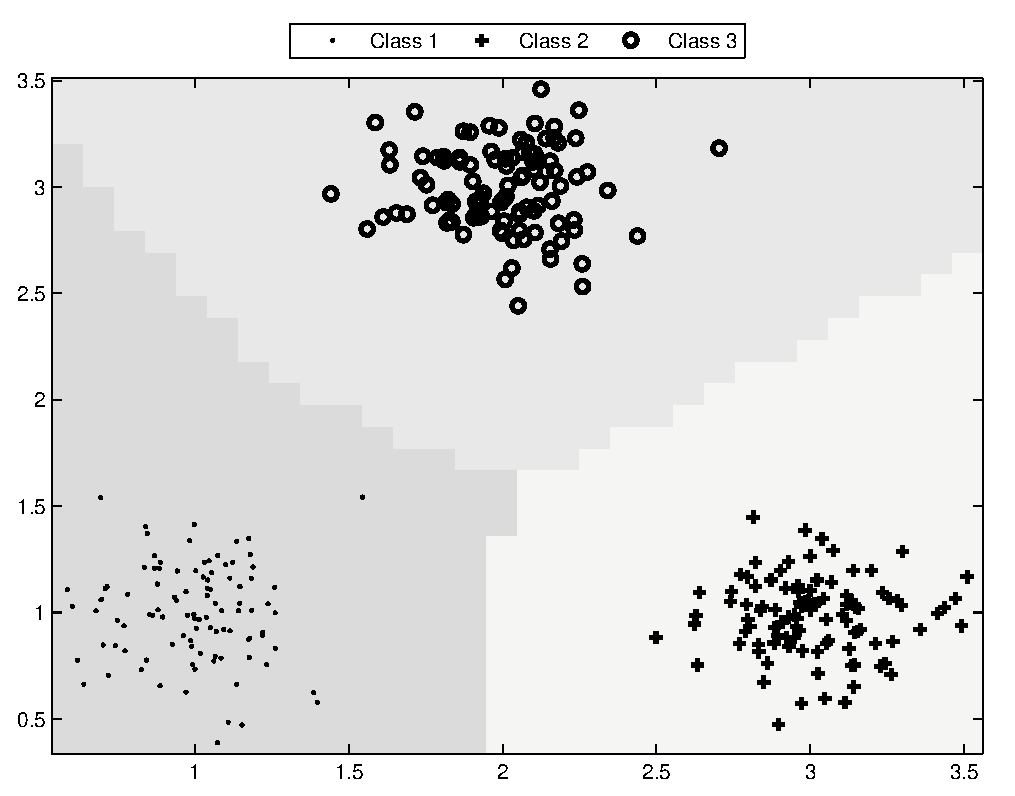
\includegraphics[scale=0.25]{{../eps/fig2_H4_eta0.010000}.eps}
\subcaption{ $H=4$}
\endminipage\hfill
\minipage{0.32\textwidth}
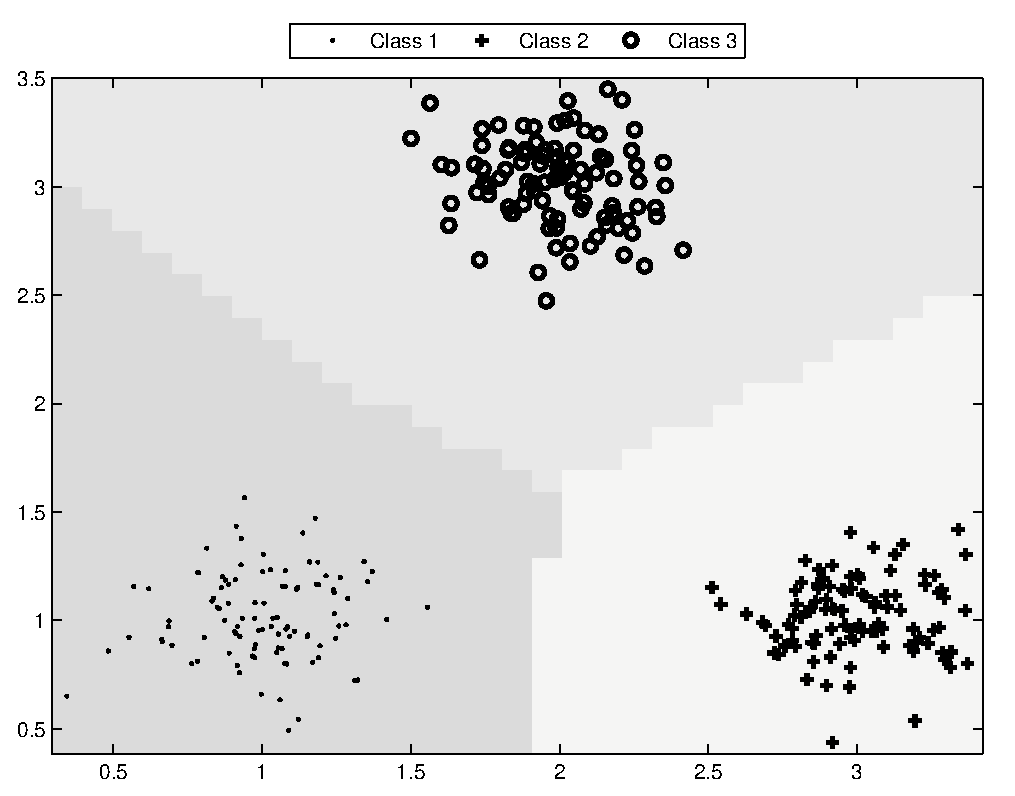
\includegraphics[scale=0.25]{{../eps/fig2_H64_eta0.010000}.eps}
\subcaption{ $H=64$}
\endminipage\hfill
\caption{Deicision boundary for $\eta=0.01$}
\label{fig:fig12}
\end{figure}

\begin{figure}[H]
\minipage{0.32\textwidth}
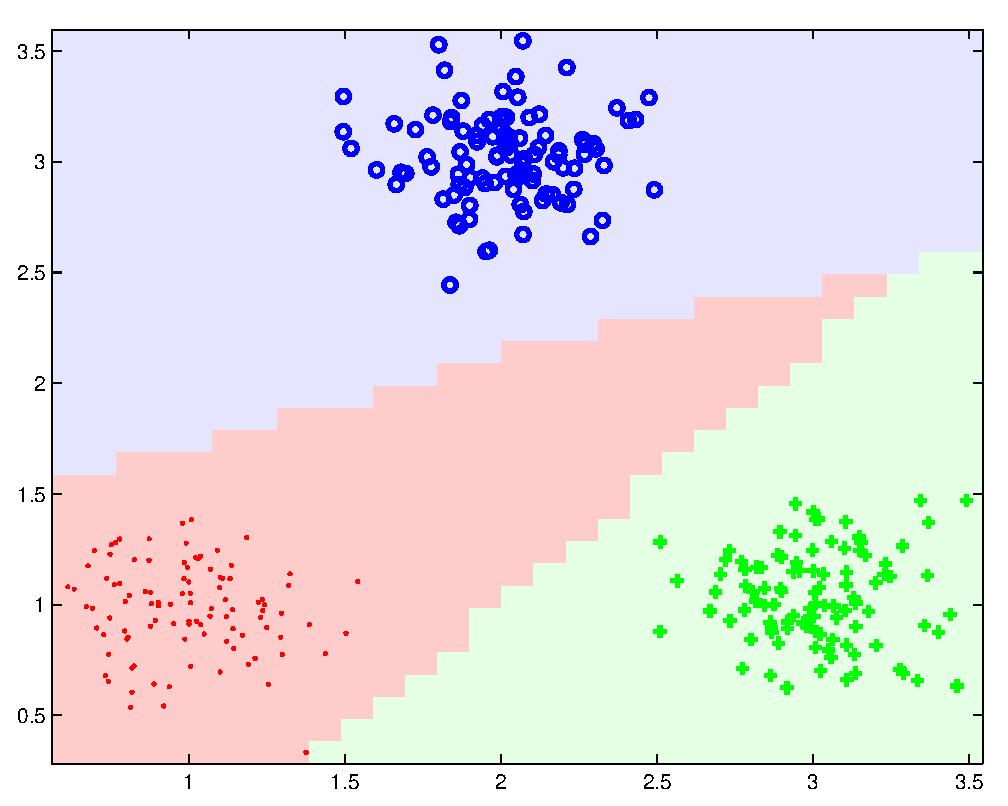
\includegraphics[scale=0.25]{{../eps/fig2_H2_eta0.001000}.eps}
\caption{ $H=2$}
\endminipage\hfill
\minipage{0.32\textwidth}
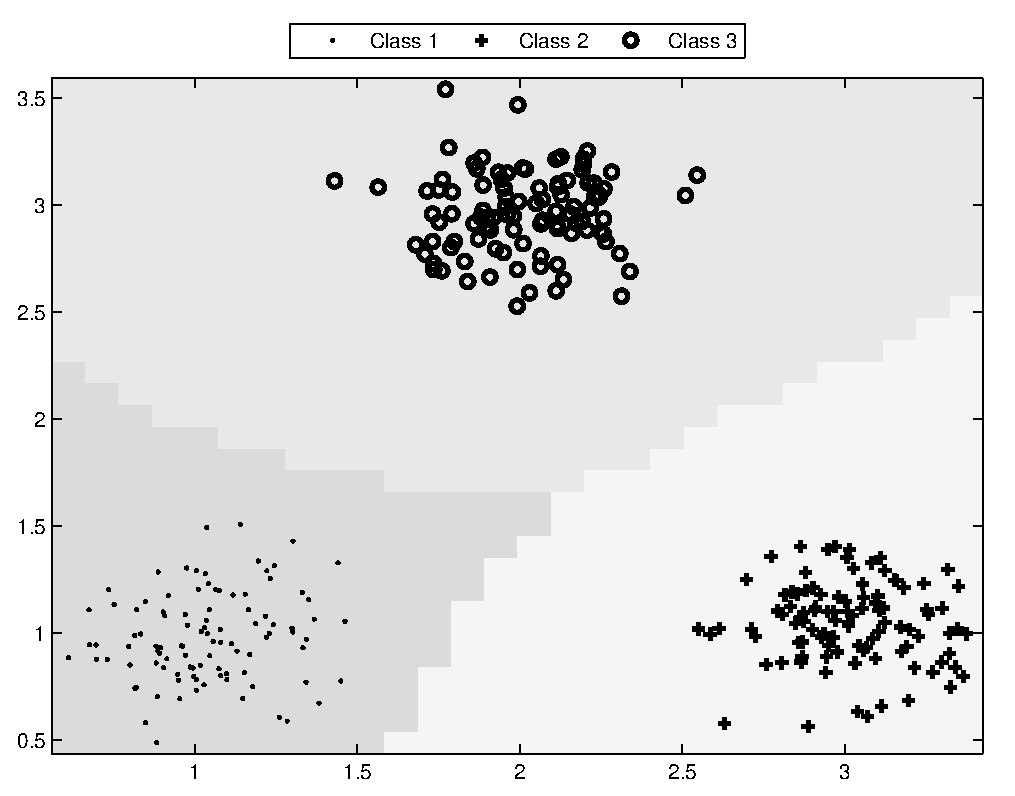
\includegraphics[scale=0.25]{{../eps/fig2_H4_eta0.001000}.eps}
\caption{ $H=4$}
\endminipage\hfill
\minipage{0.32\textwidth}
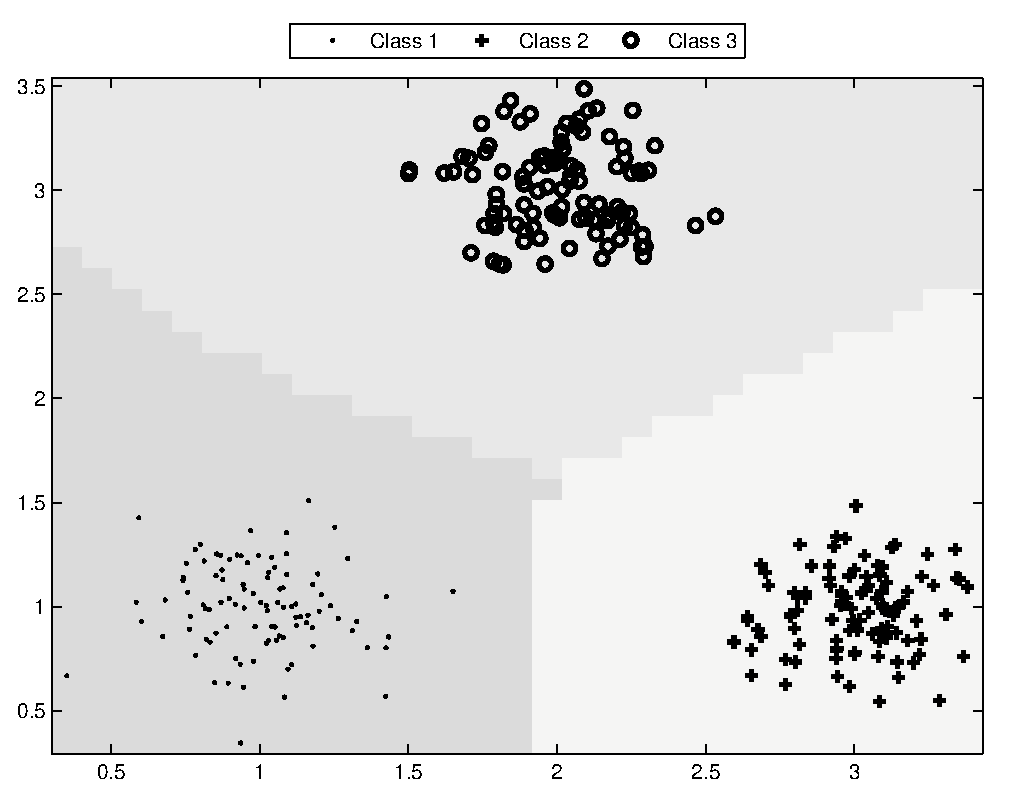
\includegraphics[scale=0.25]{{../eps/fig2_H64_eta0.001000}.eps}
\caption{ $H=64$}
\endminipage\hfill
\caption{Deicision boundary for $\eta=0.001$}
\label{fig:fig13}
\end{figure}

\begin{figure}[H]
\minipage{0.32\textwidth}
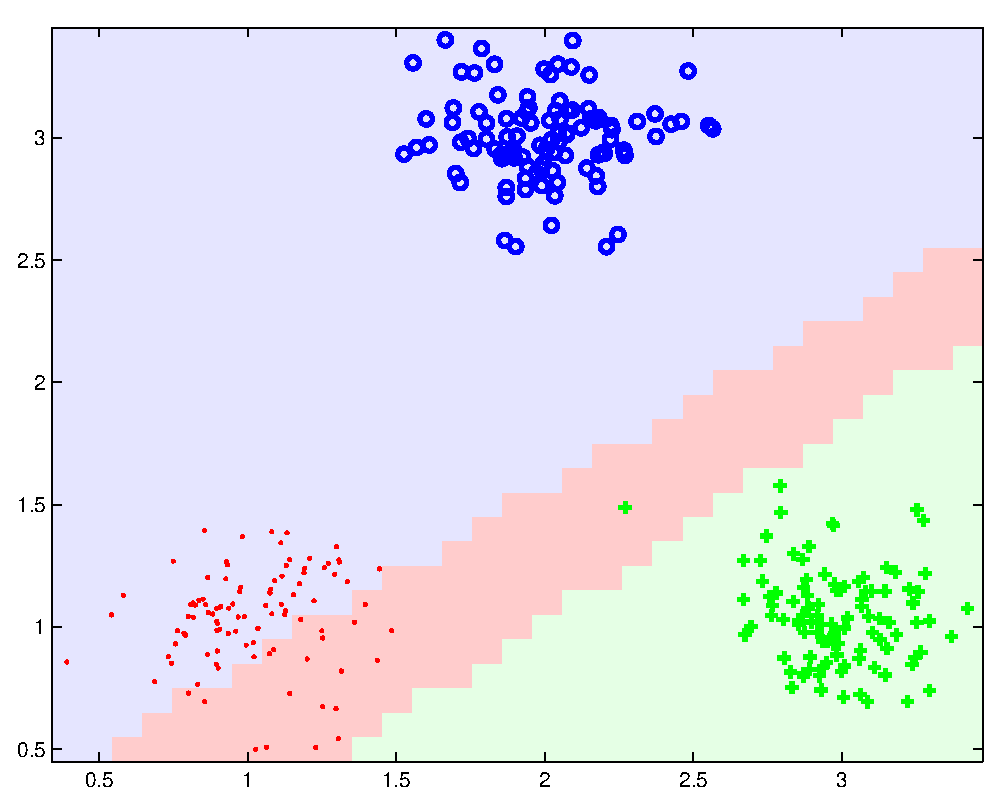
\includegraphics[scale=0.25]{{../eps/fig2_H2_eta0.000100}.eps}
\caption{ $H=2$}
\endminipage\hfill
\minipage{0.32\textwidth}
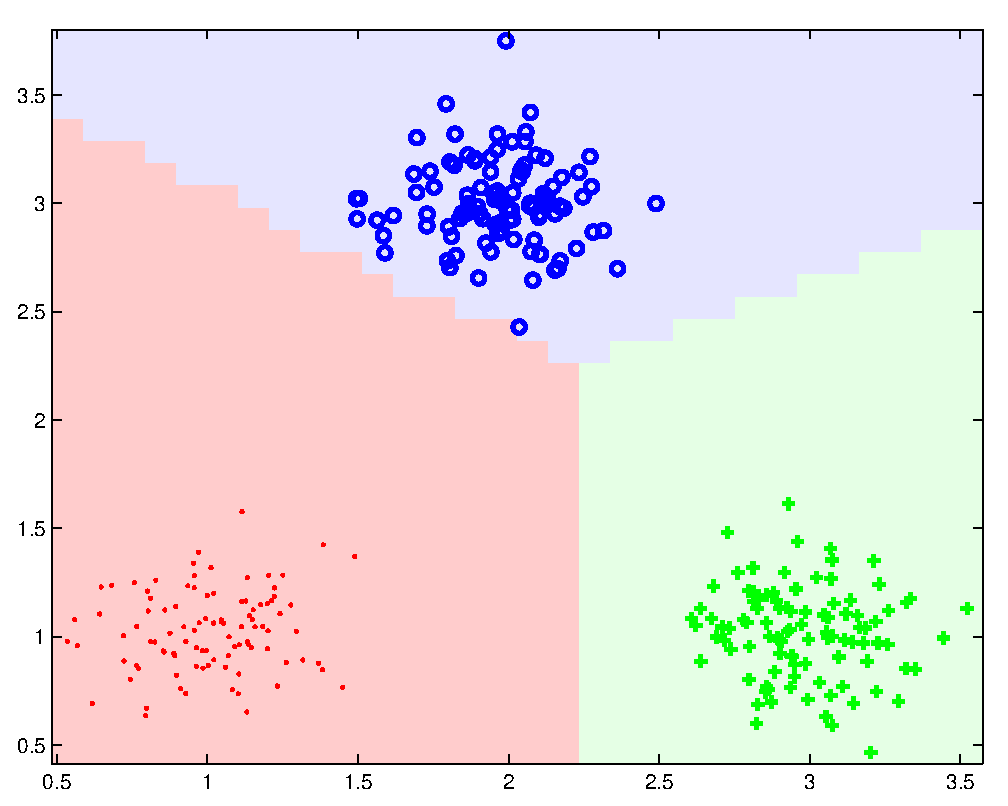
\includegraphics[scale=0.25]{{../eps/fig2_H4_eta0.000100}.eps}
\caption{ $H=4$}
\endminipage\hfill
\minipage{0.32\textwidth}
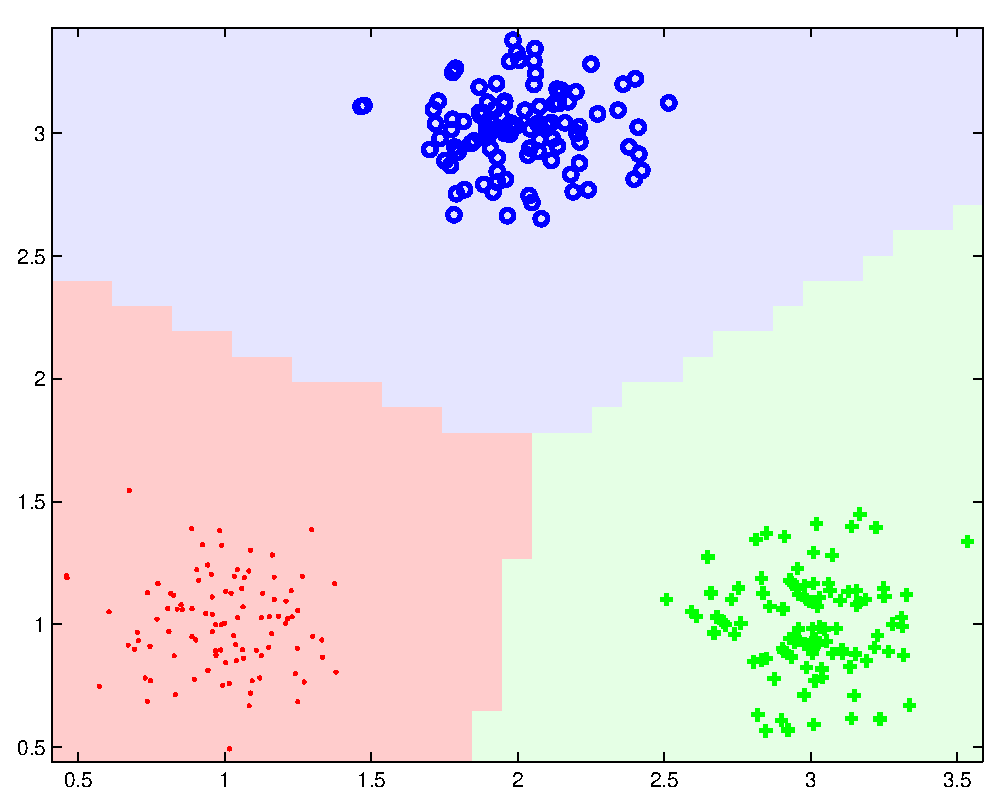
\includegraphics[scale=0.25]{{../eps/fig2_H64_eta0.000100}.eps}
\caption{ $H=64$}
\endminipage\hfill
\caption{Deicision boundary for $\eta=0.0001$}
\label{fig:fig14}
\end{figure}

\begin{figure}[H]
\minipage{0.32\textwidth}
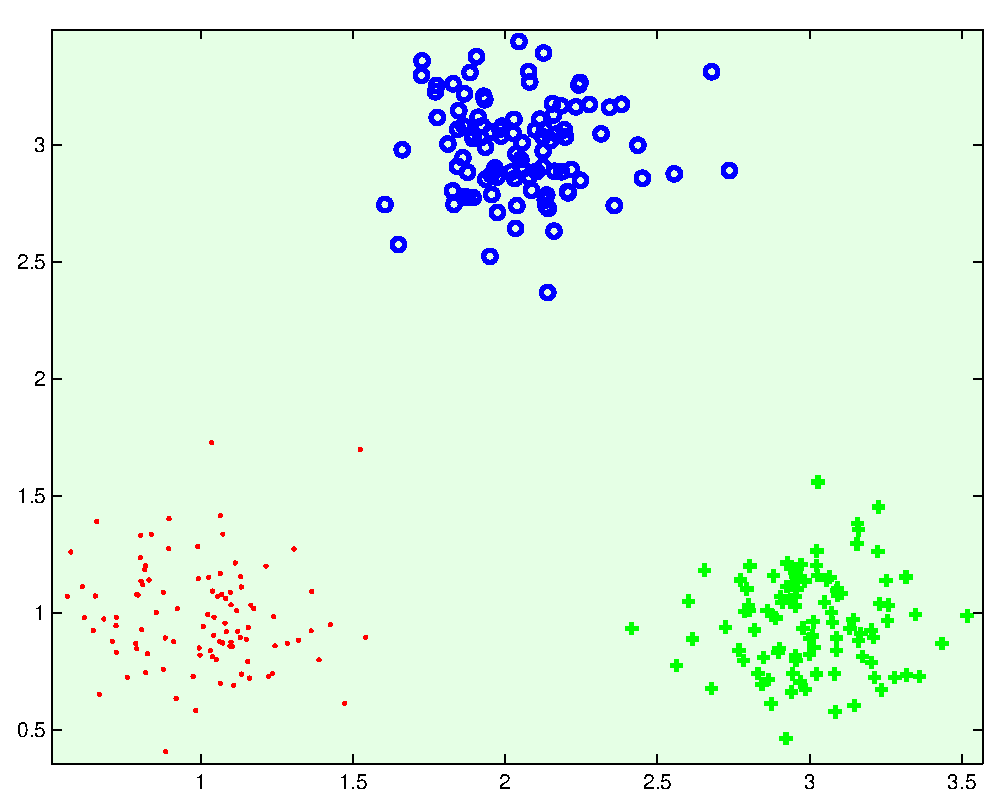
\includegraphics[scale=0.25]{{../eps/fig2_H2_eta0.000010}.eps}
\caption{ $H=2$}
\endminipage\hfill
\minipage{0.32\textwidth}
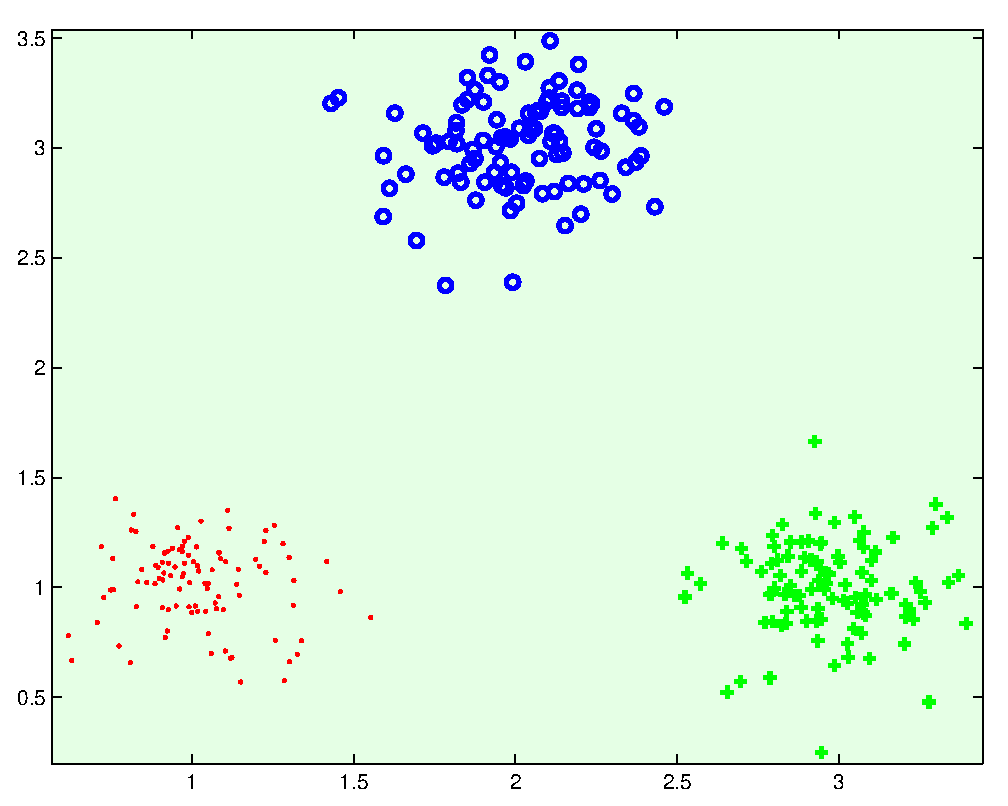
\includegraphics[scale=0.25]{{../eps/fig2_H4_eta0.000010}.eps}
\caption{ $H=4$}
\endminipage\hfill
\minipage{0.32\textwidth}
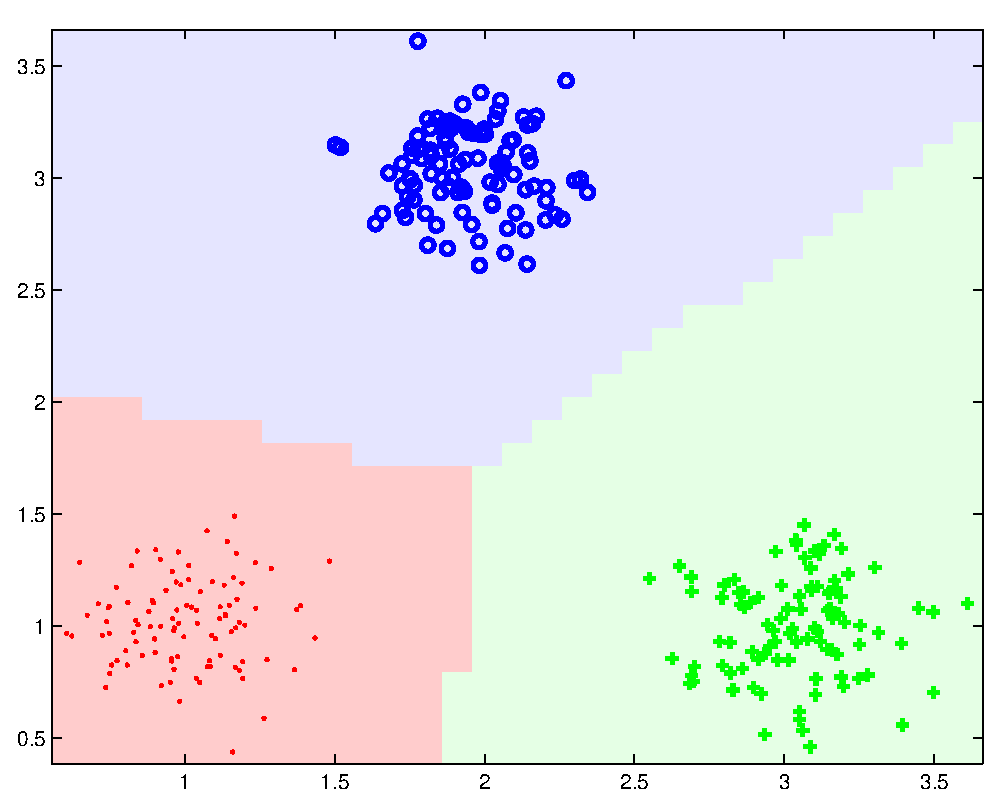
\includegraphics[scale=0.25]{{../eps/fig2_H64_eta0.000010}.eps}
\caption{ $H=64$}
\endminipage\hfill
\caption{Deicision boundary for $\eta=0.00001$}
\label{fig:fig15}
\end{figure}

\subsection{Discussion and Conclusions}
\subsubsection{Hidden Layer Nodes}
As we can see from Figure \ref{fig:fig1} and \ref{fig:fig2} increasing the number of hidden layer nodes increases the convergence rate for the neural network but in the end, all the networks become almost the same given sufficient iterations, although $H=64$ still dominates in all cases. However, in case of lower learning rate, networks with more number of hidden layer nodes are able to converge quickly in comparison to others as can be seen in Figures \ref{fig:fig3}, \ref{fig:fig4} and \ref{fig:fig5}. This is because the network will be able to represent more complex data with an increase in the number of hidden layer nodes which will represent various intermediate functions and representation of-of data (i.e. classification into classes) can be done quickly with more hidden layer nodes rather than taking more iterations with less number of hidden layer nodes. Also, this process will saturate and beyond a particular limit increasing the hidden layer nodes will not make any significant difference.

\subsubsection{Learning Rate}
As we can see from Figure \ref{fig:fig6}, \ref{fig:fig7}, \ref{fig:fig8}, \ref{fig:fig9}, \ref{fig:fig10} and \ref{fig:fig11}; increasing the learning rate leads to faster convergence. This is because the magnitude of the learning rate hasn't been too high to cause oscillations in the error space and hence increasing the learning rate within particular limits will only fasten the process of convergence of the network to a better solution.

\subsubsection{Training Iterations}
We are performing a stochastic gradient descent on the data which is based on finding the gradient with respect to a particular point and changing weights accordingly, this method will give better and better results as network is trained with more and more number of points, i.e. with increase in total iterations the error in the output of the network decreases as can be seen in all the Figures.

\subsubsection{Decision Boundary}
As we can see for appropriate learning rate all networks (i.e. varying them respect to the number of hidden layer nodes) give a very accurate description of decision boundary though they differ slightly in term of the structure and also the sum of squared errors. The reason for the latter is of the ability of networks with more complexity (more hidden layer nodes) give very strong probabilities in terms of output in case of the three classes whereas weaker networks give only mild probabilities everywhere, though the separating boundary can still remain same. We can also that though correct, weaker networks are ``unsure'' about their decision or are ``indecisive'' in cases. Also, here network with higher hidden layer nodes were able to get a nice decision boundary for even low learning rate as can be seen from Figures \ref{fig:fig12}, \ref{fig:fig13}, \ref{fig:fig14} and \ref{fig:fig15}. 

\section{Neural Network to predict the steering angle from the road image for a self-driving car}
\subsection{Network Structure}
If we consider the network to be composed of $n_1, n_2, ... n_k$ nodes in each layer with the corresponding vectors to be $\vec v_1,\vec v_2, ... \vec v_k$ and the weights for each layer be $ \vec w_1, \vec w_2, ... \vec w_{k-1}$, we can then say that $v_{ij}=\sigma(\vec w_{i-1,j}^T \vec v_{i-1}), i\in\{2,3,..k\}$. In other words: 
\begin{gather*}
\vec v_i=\begin{pmatrix}v_{i,1}\\v_{i,2}\\...\\v_{i,n_i}\end{pmatrix}_{n_i\times1},
\vec w_{i,j}=\begin{pmatrix}w_{i,1,j}\\w_{i,2,j}\\...\\w_{i,n_i,j}\end{pmatrix}_{n_i\times 1}\\
\vec w_{i}=\begin{pmatrix}\vec w_{i,1}^T\\\vec w_{i,2}^T\\...\\\vec w_{i,n_{i+1}}^T\end{pmatrix}_{n_{i+1}\times n_i}=\begin{pmatrix}w_{i,1,1}&w_{i,2,1}&...&w_{i,n_{i},1}\\w_{i,1,2}&w_{i,2,2}&...&w_{i,n_{i},2}\\\vdots&\vdots&\ddots&\vdots\\w_{i,1,n_{i+1}}&w_{i,2,n_{i+1}}&...&w_{i,n_i,n_{i+1}}\end{pmatrix}
\end{gather*}
where
\begin{align*}
\vec v_i&\text{ is Layer $i$}\\
v_{i,j}&\text{ is $j^\text{th}$ node in Layer $i$}\\
\vec w_i&\text{ is weight from Layer $i$ to $i+1$}\\
\vec w_{i,j}&\text{ is weight from Layer $i$ to $j^\text{th}$ node in Layer $i+1$}\\
w_{i,a,b}&\text{ is weight from $a^\text{th}$ node in Layer $i$ to $b^\text{th}$ node in Layer $i+1$}
\end{align*}
and thus
\begin{align*}
v_{i,j} &=\begin{cases}\sigma(\vec w_{i-1,j}^T\vec v_{i-1})&i\ne k\\\vec w_{k-1,j}^T\vec v_{k-1}&i=k\end{cases}
\end{align*}
and therefore
\begin{align*}
\vec v_i= \begin{cases}\vec \sigma (\vec w_{i-1}\vec v_{i-1})&i\ne k-1\\\vec w_{k-1}\vec v_{k-1}&i=k\end{cases}
\end{align*}

\begin{figure}[H]
\centering
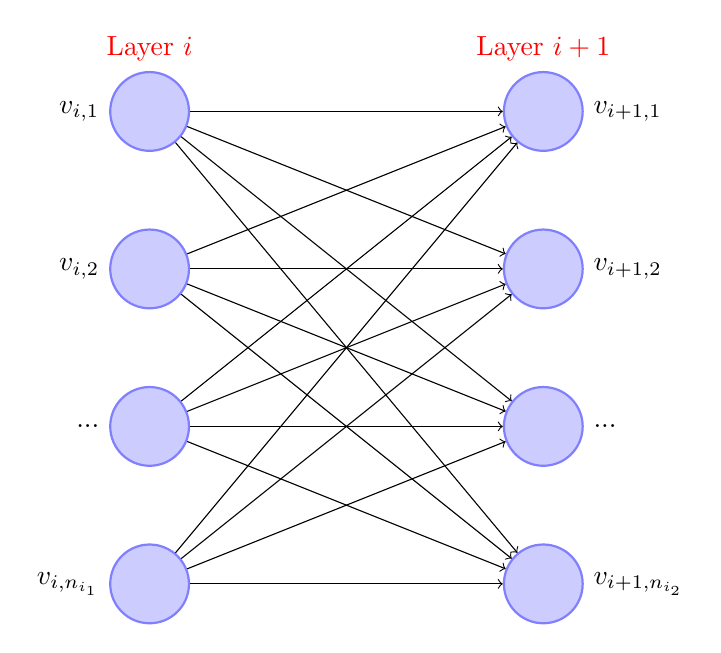
\begin{tikzpicture}
[auto, nd/.style = {circle,minimum size=1cm,draw=blue!50,fill=blue!20,thick}]

\foreach \n/\name in {1/1,2/2,3/x,4/{$n_{i_1}$}}
		\node[nd] (I\n) at (0,-2*\n) [label=left:{ \ifthenelse{\equal{\name}{x}}{{...}}{$v_{i,\text{\name}}$} }] {};
		
\foreach \n/\name in {1/1,2/2,3/x,4/{$n_{i_2}$}}
		\node[nd] (J\n) at (5,-2*\n) [label=right:{ \ifthenelse{\equal{\name}{x}}{{...}}{$v_{i+1,\text{\name}}$} }] {};		
		
\foreach \i/\o in {1/1,2/2,3/x,4/{$n_1$}}{
	\foreach \j/\k in {1/1,2/2,3/x,4/{$n_2$}}{
		\draw [->] (I\i) -- (J\j);
	}
}

\node[red,above] at (I1.north) {Layer $i$};
\node[red,above] at (J1.north) {Layer $i+1$};

\end{tikzpicture}
\caption{Portion of a neural network from layer $i$ to layer $i+1$. The weight used here will be $\vec w_i$.}
\end{figure}
\subsection{Gradient Descent}
The error term for a minibatch of size $n$ (i.e. from $j$ to $j+n-1$) would be:
$$E = \sum_{i=j}^{j+n-1}\frac 12 || \vec o^i- \vec v_{k}^i||^2$$
where superscript $i$ denotes the $i$-th point.
For a particular point the error would be:
$$\frac 12 || \vec o- \vec v_{k}||^2=\frac 12\sum_{l=1}^{n_k}(o_{l}-v_{k,l})^2$$
The gradient wrt weights $w_{k-1,a_{k-1},a_{k}}$ can be obtained using chain rule:\\
$$\frac{\partial E}{\partial w_{k-1,a_{k-1},a_{k}}}=\underbrace{(v_{k,a_k}-o_{a_k})}_{\delta_{k,a_k}}v_{k-1,a_{k-1}}$$
Similarly for any previous layer we can obtain:\\
$$\frac{\partial E}{\partial w_{i,a_i,a_{i+1}}}=\underbrace{v_{i+1,a_{i+1}}(1-v_{i+1,a_{i+1}})\sum_{a_{i+2}=1}^{n_{i+2}} \delta_{i+2,a_{i+2}}w_{i+1,a_{i+1},a_{i+2}}}_{\delta_{i+1,a_{i+1}}}v_{i,a_i}$$
and wrt a particular point\\
$$\Delta w_{i,a_i,a_{i+1}}=\eta \delta_{i+1,a_{i+1}}v_{i,a_i}$$
For minibatch gradient descent we would add up these $\Delta w_{i,a_i,a_{i+1}}$'s. Also note that we also have some biases that would not propagate the gradient backwards so in case of calculation of $\delta_{i,a_i}$ we would neglect the term coming from $v_{a_{i+1}}=1$ i.e. the bias term of the $i+1$-th layer.

Now we find a relation between $\delta_{i,j}$'s. We define $\vec \delta_i$ as follows:
$$\vec \delta_i=\begin{pmatrix}\delta_{i,1}\\\delta_{i,2}\\...\\\delta_{i,n_i}\end{pmatrix}_{n_i\times 1}$$
And we define $\delta_{i,j}$ as follows:
$$\delta_{i,j}=\begin{cases}v_{k,j}-o_j&i=k\\\displaystyle v_{i,j}(1-v_{i,j})\sum_{x=1}^{n_{i+1}}\delta_{i+1,x}w_{i,j,x}&\text{otherwise}\end{cases}$$
We can observe that:
\begin{gather*}\Delta\vec w_{i}=\eta \vec \delta_{i+1}\vec v_{i}^T\\
\vec\delta_i=\begin{cases}\vec v_i \circ (\vec 1-\vec v_i)\circ \vec w_i^T\vec \delta_{i+1}&i\ne k\\\vec v_k-\vec o&i=k\end{cases}
\end{gather*}
where $(\circ)$ is the elementwise product.
\subsection{Minibatch gradient Descent}
We define few more quantities (here superscript $i$ denotes $i$-th point, $n$ denotes total points in a minibatch):
\begin{gather*}
\vec V_i = \begin{pmatrix}\vec v_i^1&\vec v_i^2&...&\vec v_i^n\end{pmatrix}\\
\vec O = \begin{pmatrix}\vec o^1&\vec o^2&...&\vec o^n\end{pmatrix}\\
\vec \xi_i =\begin{pmatrix}\vec \delta_i^1&\vec \delta_i^2&...&\vec \delta_i^n\end{pmatrix}
\end{gather*}
We note that:
\begin{gather*}
\vec V_i = \begin{cases}\vec \sigma (\vec w_{i-1}\vec V_{i-1})&i\ne k-1\\ \vec w_{k-1}\vec V_{k-1}&i=k\end{cases}\\
\vec \xi_i = \begin{cases}\vec V_i\circ (\vec 1-\vec V_i)\circ\vec w_i^T\vec \xi_{i+1}&i\ne k\\\vec V_k-\vec O&i=k\end{cases}\\
\Delta \vec w_i = \eta\vec \xi_{i+1} \vec V_{i}^T=\eta \sum_{j=1}^n\vec \delta_{i+1}^j\vec v_i^{j,T}
\end{gather*}
\subsection{Dropout}
For implementation of dropout, some of the nodes in the layers $V_1$ to $V_{k-1}$ are disabled with probability $p$ (say $0.5$), thus the modified layer vectors would become:
\begin{gather*}
V_i'=V_i\circ D_i\tag{$i<k$}
\end{gather*}
where $D_i$ is a matrix of independent Bernoulli random variables with probability $p$, i.e. $(D_i)_{\alpha,\beta}\sim{\rm Bernoulli}(p), 1\le \alpha \le n_i, 1\le \beta \le n$ (recall $n$ is minibatch size) and of the same size as of $V_i$. During backpropagation, the $\xi$ values are modified with the same $D_i$ as:
\begin{align*}
\xi_i'&=\xi_i\circ D_i \\&= V_i' \circ (1-V_i') \circ \vec w_i^T\vec \xi_{i+1}\;'\circ D_i\\\tag{$i<k$}
&=(D_i\circ V'_i)\circ (1-V_i') \circ \vec w_i^T\vec \xi_{i+1}\;'\\
&=V_i'\circ (1-V_i') \circ \vec w_i^T\vec \xi_{i+1}\;'\\
&=\xi_i
\end{align*}
We note that for $i<k$, the $\xi_i$ terms already include $D_i$'s whose inclusion further doesn't make any change so we don't need to change anything in the backpropagation. We further note that:
\begin{itemize}
\item The bias term is not multiplied with $D_i$.
\item At testing we multiply the weights by $p$ and the network is used without dropout.
\end{itemize}
\subsection{Observations}
The following graphs were observed
\subsubsection{Training for $5000$ epochs at $\eta=0.01$ without dropout}
\begin{figure}[H]
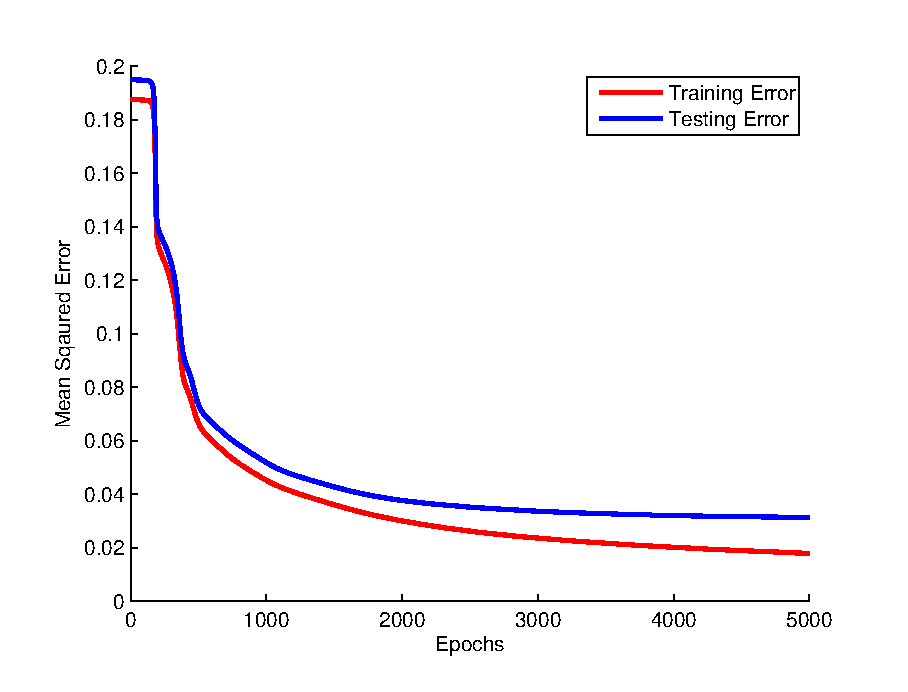
\includegraphics[scale=\myScale]{../q2/part1}
\caption{Variation of Training and Testing error as a function of number of epochs with parameters $\eta=0.01$, architecture $[1024,512,64,1]$, split ratio $0.8$, epochs $5000$, minibatch size $64$, dropout rate $0$.}
\label{fig:fig16}
\end{figure}
\subsubsection{Varying minibatch size}
\begin{figure}[H]
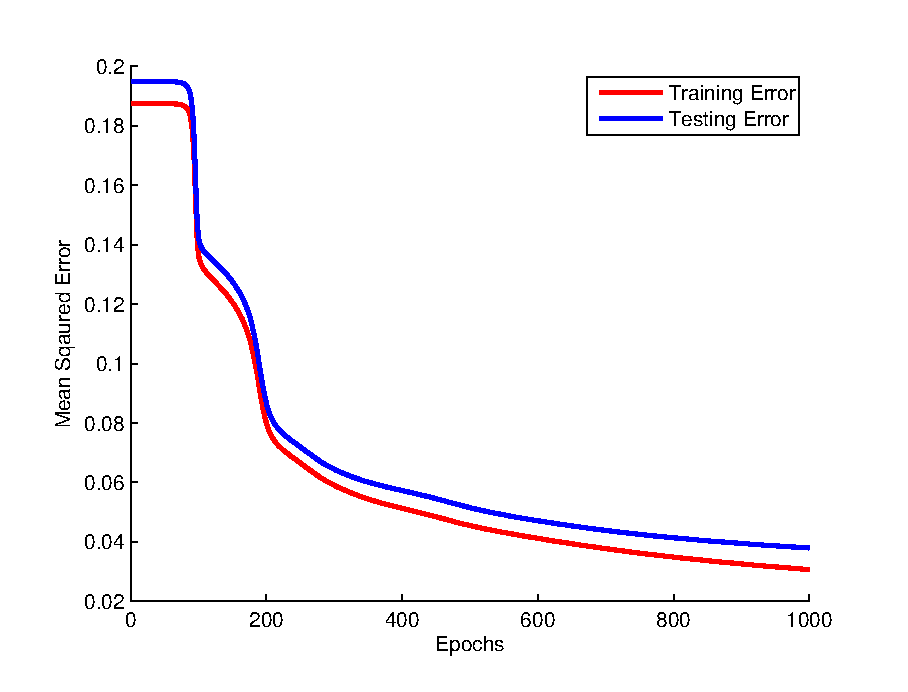
\includegraphics[scale=\myScale]{../q2/part2_32}
\caption{Variation of Training and Testing error as a function of number of epochs with parameters $\eta=0.01$, architecture $[1024,512,64,1]$, split ratio $0.8$, epochs $1000$, {\bf minibatch size $32$}, dropout rate $0$.}
\label{fig:fig17}
\end{figure}
\begin{figure}[H]
\includegraphics[scale=\myScale]{../q2/part2_64}
\caption{Variation of Training and Testing error as a function of number of epochs with parameters $\eta=0.01$, architecture $[1024,512,64,1]$, split ratio $0.8$, epochs $1000$, {\bf minibatch size $64$}, dropout rate $0$.}
\label{fig:fig18}
\end{figure}
\begin{figure}[H]
\includegraphics[scale=\myScale]{../q2/part2_128}
\caption{Variation of Training and Testing error as a function of number of epochs with parameters $\eta=0.01$, architecture $[1024,512,64,1]$, split ratio $0.8$, epochs $1000$, {\bf minibatch size $128$}, dropout rate $0$.}
\label{fig:fig19}
\end{figure}
\subsubsection{Dropout}
\begin{figure}[H]
\includegraphics[scale=\myScale]{plot_04_11_14_52}
\caption{Variation of Training and Testing error as a function of number of epochs with parameters {\bf learning rate $\eta=0.001$}, architecture $[1024,512,64,1]$, split ratio $0.8$, epochs $1000$, minibatch size $64$, {\bf dropout rate $0.5$}.}
\label{fig:fig20}
\end{figure}
\begin{figure}[H]
\includegraphics[scale=\myScale]{plot_04_11_16_50}
\caption{Variation of Training and Testing error as a function of number of epochs with parameters {\bf learning rate $\eta=0.005$}, architecture $[1024,512,64,1]$, split ratio $0.8$, epochs $1000$, minibatch size $64$, {\bf dropout rate $0.5$}.}
\label{fig:fig21}
\end{figure}
\begin{figure}[H]
\includegraphics[scale=\myScale]{plot_04_11_18_33}
\caption{Variation of Training and Testing error as a function of number of epochs with parameters {\bf learning rate $\eta=0.01$}, architecture $[1024,512,64,1]$, split ratio $0.8$, epochs $1000$, minibatch size $64$, {\bf dropout rate $0.5$}.}
\label{fig:fig22}
\end{figure}
\subsubsection{Varying Learning Rate}
\begin{figure}[H]
\includegraphics[scale=\myScale]{../q2/part4_0p005}
\caption{Variation of Training and Testing error as a function of number of epochs with parameters {\bf learning rate $\eta=0.005$}, architecture $[1024,512,64,1]$, split ratio $0.8$, epochs $1000$, minibatch size $128$, dropout rate $0$.}
\label{fig:fig23}
\end{figure}
\begin{figure}[H]
\includegraphics[scale=\myScale]{../q2/part4_0p001}
\caption{Variation of Training and Testing error as a function of number of epochs with parameters {\bf learning rate $\eta=0.001$}, architecture $[1024,512,64,1]$, split ratio $0.8$, epochs $1000$, minibatch size $128$, dropout rate $0$.}
\label{fig:fig24}
\end{figure}
\begin{figure}[H]
\includegraphics[scale=\myScale]{../q2/part4_0p05}
\caption{Variation of Training and Testing error as a function of number of epochs with parameters {\bf learning rate $\eta=0.05$}, architecture $[1024,512,64,1]$, split ratio $0.8$, epochs $1000$, minibatch size $128$, dropout rate $0$.}
\label{fig:fig25}
\end{figure}
\subsection{Conclusions and Discussions}
The result for a particular set of parameters has provided the corresponding graph. It is observed at first that the mean of the sum of the squared error decreases slowly and then has a sudden drop in its values. This trend continues for a short while before the decrease becomes more gradual, and finally the rate of decrease is almost null, providing us with the final value of the error. This is justifiable as the network learns more values, the network learns to clasify more properly leading to a rapid decrease in error untill it reaches a point from where the deacrease rate is gradual. Moreover the testing set error at the end is more than the traing error as their is some amount of overfitting due to the training set, in the network learned.

\subsubsection{Learning Rate}
As observed from the graphs for various learning rates, it is seen that higher the learning rate, lower is the mean of the sum of squared error for both training and testing data. This is very much justifiable as a larger learning rate tends to represent a higher possibility of change in the way the neural network learns the dataset  with respect to the change in the dateset. Lower learning rate takes a longer time to converge with respect to higher learning rate, which converges better. However if given enough time the error value for lower learning rate is lower that its higer learning rate counterpart.


\subsubsection{Minibatch Size}
As observed from the graphs for various minibatch size, it is seen that lower the minibatch size, lower is the mean of the sum of squared error for both training and testing data. Also if minbatch size is taken as one it would land up being stocastic gradient descent. This will require for frequent updates causing the error to decrease more. Therefore for larger minibatch size the no of updates would be relatively low causing the overall error value to be relatively highre than lower minibatch size.

\subsubsection{Dropout}
As observed from the graphs for various dropout rates it has been observed that for a particular dropout rate increasing the learning rate increases the fluctuations in the mean of the sum of squared error for both training and testing data. As for lower learning rate the mean of the sum of squared error deacreases first then fluctuates very little about a value giving almost a straight line. It has also been observed that for a particular learning rate having a dropout ( here it is $0.5$ ) has lead to the increase in the mean of the sum of squared error than when there was no dropout at all.

\section{Improved network for steering angle prediction}
\subsection{Network Structure}
The network structure was composed of $[512-64-1]$ with $\eta =0.05$ and minibatch size $32$. A not so optimum result was also obtained using a convolutional neural network
\begin{itemize}
\item Input of size $32\times32\times 1$
\item 3D Convolutional Layer with $8$ filters of size $3\times3\times1$ which gives $8$ feature maps of size $30\times30$ (RELU activation)
\item 3D Convolutional Layer with $4$ filters of size $3\times3\times32$ which gives $4$ feature maps of size $28\times28$ (RELU activation)
\item Max Pooling layer of size $2\times 2$ with stride $2$ applied to each feature map independently gives $4$ feature maps of size $14\times14$
\item Flattening of these to a layer of size $784$
\item Dense layer of size $512$ (Sigmoid activation)
\item Dense layer of size $64$ (Sigmoid activation)
\item Output layer of size $1$ (Linear activation)
\end{itemize}
\subsubsection{Convolution Layer}
Suppose we have an image$I$ of size $H\times W$ with pixels $x_{i,j}$ which is cross-correlated with a kernel $K$ with weights $w_{i,j}$ of size $k_1\times k_2$ with bias $b$ and an activation $f$, then the resultant image has the pixels:
$$(I*K)_{i,j}=x'_{i,j}=\sum_{m=0}^{k_1-1}\sum_{n=0}^{k_2-1}x_{i+m,j+n}w_{m,n}+b$$
and after activation:
$$o'_{i,j}=f(x'_{i,j})$$
Let us find the weight update equations with $t$ as target value and $o^k$ as the predicted value (output at $k$-th layer), the given error is:
$$E=\frac 12\sum ||t-o^k||^2$$
and therefore for a resultant image of size $(H-k_1+1)\times(W-k_2+1)$ (here superscripts denote the layer index):
\begin{align*}
\frac{\partial E}{\partial w_{m',n'}^l} &= \sum_{i=0}^{H-k_1}\sum_{j=0}^{W-k_2}\underbrace{\frac {\partial E}{\partial x_{i,j}^{l}}}_{\delta_{i,j}^{l}}\frac{\partial x_{i,j}^{l}}{\partial w_{m',n'}^l}\\
&= \sum_{i=0}^{H-k_1}\sum_{j=0}^{W-k_2}\delta_{i,j}^{l}\frac{\partial}{\partial w_{m',n'}^l}\left(\sum_{m=0}^{k_1}\sum_{n=0}^{k_2} w_{m,n}^lo_{i+m,j+n}^{l-1}+b^l\right)\\
\frac{\partial x_{i,j}^{l+1}}{\partial w_{m',n'}^l}&=\frac{\partial}{\partial w_{m',n'}^l}\left(w_{0,0}^lo_{i,j}^{l-1}+...+w_{m',n'}^lo_{i+m',j+n'}^{l-1}+...+b^l\right)\\
&=o_{i+m',j+n'}^{l-1}\\
\frac{\partial E}{\partial w_{m',n'}^l}&=\sum_{i=0}^{H-k_1}\sum_{j=0}^{W-k_2}\delta_{i,j}^{l}o_{i+m',j+n'}^{l-1}
\end{align*}
Hence we can see that the gradients are also a cross-correlation operation as follows:
$$\left(\overrightarrow{\frac{\partial E}{\partial w^l}}\right)_{i,j}=(I'*\vec \delta)_{i,j}$$
Now let us find a relation between $\delta_{i,j}^k$'s:
\begin{align*}
\delta_{i,j}^l&=\frac{\partial E}{\partial x_{i,j}^l}=\sum_{m,n}\frac{\partial E}{\partial x_{m,n}^{l+1}}\frac{\partial x_{m,n}^{l+1}}{\partial x_{i,j}^l}\\
&=\sum_{m,n}\delta_{m,n}^{l+1}\frac{\partial x_{m,n}^{l+1}}{\partial x_{i,j}^l}
\end{align*}
and hence:
\begin{align*}
\frac{\partial x_{m,n}^{l+1}}{\partial x_{i,j}^l}&=\frac{\partial }{\partial x_{i,j}^l}\left(\sum_{m'}\sum_{n'}w_{m',n'}^{l+1}o_{m+m',n+n'}^l+b^{l+1}\right)\\
&=\frac{\partial }{\partial x_{i,j}^l}\left(\sum_{m'}\sum_{n'}w_{m',n'}^{l+1}f(x_{m+m',n+n'}^l)+b^{l+1}\right)\\
&=\frac{\partial }{\partial x_{i,j}^l}\left(w_{i-m,j-n}^{l+1}f(x_{i,j}^l)\right)\\
&=w_{i-m,j-n}^{l+1}f'(x_{i,j}^l)\\
\delta_{i,j}^l&=\frac{\partial E}{\partial x_{i,j}^l}=\sum_{m,n}\delta_{m,n}^{l+1}w_{i-m,j-n}^{l+1}f'(x_{i,j}^l)
\end{align*}
We can see that this is also a cross correlation operation with weights transposed:
\begin{gather*}
\vec\delta\,^l=(\vec \delta\,^{l+1}*\vec w\,^{T,l+1})\circ \vec f'
\end{gather*}
\begin{thebibliography}{}
\bibitem{} 
\href{https://medium.com/towards-data-science/ learning-rate-schedules-and-adaptive-learning-rate-methods-for-deep-learning-2c8f433990d1}{Learning Rate Schedules and Adaptive Learning Rate Methods for Deep Learning}

 
\bibitem{} 
\href{http://www.jefkine.com/general/2016/09/05/backpropagation-in-convolutional-neural-networks/}{Backpropagation In Convolutional Neural Networks}

\bibitem{} 
\href{http://cs231n.github.io/convolutional-networks/}{Convolutional Neural Networks: Architectures, Convolution / Pooling Layers}

\bibitem{}
\href{http://cs231n.github.io/neural-networks-3/}{Neural Networks Part 3: Learning and Evaluation}

\bibitem{}
\href{https://wiseodd.github.io/techblog/2016/07/16/convnet-conv-layer/}{Convnet: Implementing Convolution Layer with Numpy}

\bibitem{}
\href{https://wiseodd.github.io/techblog/2016/07/18/convnet-maxpool-layer/}{Convnet: Implementing Maxpool Layer with Numpy}

\bibitem{}
\href{https://stackoverflow.com/questions/30109068/implement-matlabs-im2col-sliding-in-python}{Implement MATLAB's im2col ``sliding'' in Python} and \href{https://stackoverflow.com/questions/42474491/implement-matlabs-col2im-sliding-in-python}{Implement MATLAB's col2im 'sliding' in Python}
\end{thebibliography}
\end{document}